\documentclass{article}
\usepackage[utf8]{inputenc}
\usepackage[T2A]{fontenc}
\usepackage[utf8]{inputenc}
\usepackage[russian]{babel}
\usepackage[margin=3cm]{geometry}
\usepackage{paralist}
\usepackage{amsthm, amsmath, amsfonts, amssymb}
\usepackage{mathtools} % \mathclap
\usepackage{bm}
\usepackage{dsfont}
\usepackage{hyperref}
\usepackage{graphicx}
\usepackage{multirow}
\usepackage{comment}
\usepackage{xcolor, colortbl}
\usepackage{xifthen, xspace}
\usepackage{caption, subcaption}
\usepackage{lscape}
\usepackage{braket}
\usepackage{epigraph}
\usepackage{sectsty}

\title{\text{Домашняя работа №3}}
\author{\text{Шамриков Алексей А-05-19} }

\begin{document}

\maketitle
\section{Машины Тьюринга}

% ЗАДАНИЕ 1
\subsection{Операции с числами}

Реализуйте машины Тьюринга, которые позволяют выполнять следующие операции:
\begin{enumerate}
    \item Сложение двух унарных чисел
    \begin{figure}[h]
        \centering
        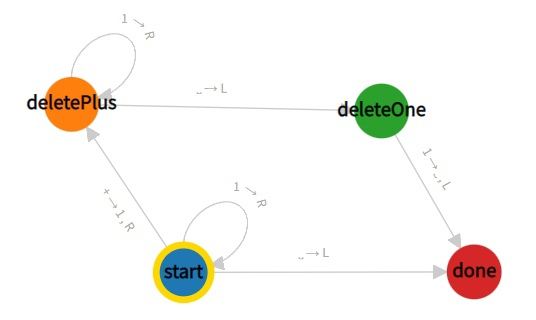
\includegraphics[width=14cm]{pictures/1.1.jpg}
    \end{figure}
\\
\ Алгоритм работы такой: проходим по ленте до конца вправо, заменив "+" на единицу. Затем, пройдя до конца, удаляем последнюю единицу. \\ \\
\ 1+1 -> 111 -> 11\\
\\
\begin{tabular}{|*{5}{c|}}
\hline
\textbf{ } & 1 & + & ' '\\
\hline\hline
q0 & <q0,x,R> & <q1,' ',R>  & <done, ' ',R> \\
\hline\hline
q1 & <q1,1,R> &  & <q2, ,L>\\
\hline\hline
q2 & <done, ,L> & & \\
\hline\hline
\hline
\end{tabular}
    \item Умножение унарных чисел
        \begin{figure}[h]
        \centering
        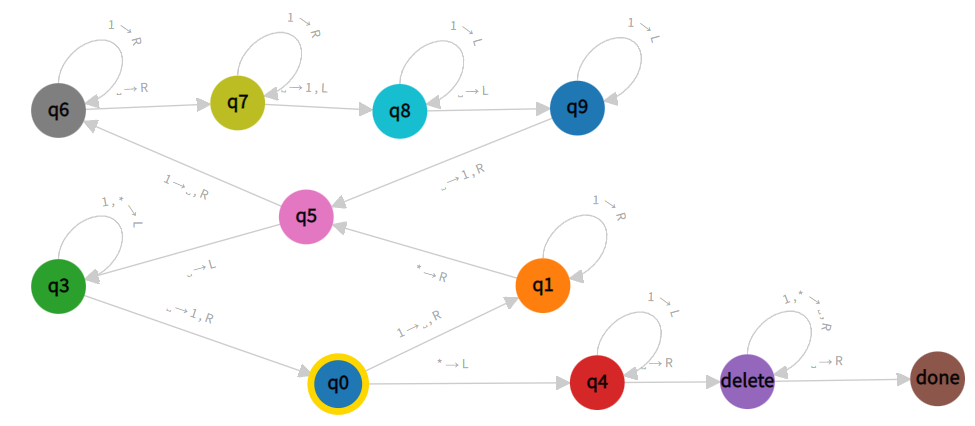
\includegraphics[width=14cm]{pictures/1.2.png}
    \end{figure}
    
\ 111*11 -> 111111\\
\\
Алгоритм:\\
Сначала мы получаем первую единицу левого множителя, очищяем ее и идем до оператора произведения.Все, что стоит за оператором мы начинаем переносить вправо по такому принципу: между начальной строкой и скопированными единицами должен быть разделительный пробел. Когда мы переносим единицу, мы оцищаем клетку, однако мы восполяем ее снова, когда начинаем переносить следующую единицу. Когда мы полснотью скопировали правый множитель, мы возвращаемся к первому, восстанавливая первую его единицу и очищая вторую. Так происходит до тех пор, пока мы не пройдем весь левый множитель. Затем мы очищаем все, что находится левее разделительного пробела. \\
\\
\begin{tabular}{|*{4}{c|}}
\hline
\textbf{ } & 1 & * & ' '\\
\hline\hline
q0 & <q1, ,R> & <q4,1,L> & \\
\hline\hline
q1 & <q1,1,R> & <q5,*,R> & \\
\hline\hline
q3 & <q3,1,L> & <q3,*,L> &\\
\hline\hline
q4 & <q4,1,L> & & <delete,' ',R>\\
\hline\hline
q5 & <q6, ,R> & &\\
\hline\hline
q6 & <q6,1,R> & & <q7, ,R> \\
\hline\hline
q7 & <q7,1,R> & & <q8,1,L> \\
\hline\hline
q8 & <q8,1,L> &  & <q9, ,L> \\
\hline\hline
q9 & <q9,1,L> & & <q5,1,R> \\
\hline\hline
delete & <delete, , R> & <delete, , R> & <done, ,R>\\
\hline
\end{tabular}
\end{enumerate} \\ \\
% КОНЕЦ ЗАДАНИЯ 1
\\ \\ 
% НАЧАЛО ЗАДАНИЯ 2
\subsection{Операции с языками и символами}

Реализуйте машины Тьюринга, которые позволяют выполнять следующие операции:
\begin{enumerate}
    \item Принадлежность к языку $L = \{ 0^n1^n2^n \}, n \ge 0$
    \begin{figure}[h]
        \centering
        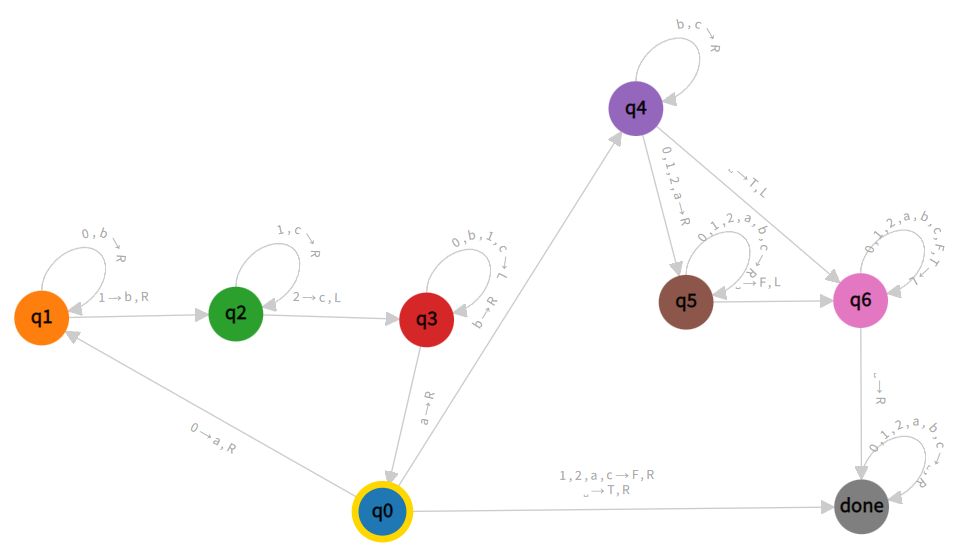
\includegraphics[width=16cm]{pictures/2.1.png}
    \end{figure}
    \\ \\ \\ \\ \\ \\ \\ 
\ Примеры:\\
\ 001122 -> T \\
\ 012 -> T \\
\ 001122 -> T \\
\ 000111222 -> T \\
\ 000011112222 -> T\\
\ 00011222 -> F\\
\ 000122 -> F\\
\\ \\
Алгоритм:\\
Проходим по ленте n раз, заменяя нули на a, единицы на b и двойки на c, причем за один проход мы заменяем только один ноль, одну единицу и одну двойку. Если оказывается, что все единицы и двойки уже были заменены, а нули - нет, тогда мы сразу переходим в терминальное состояние, записывая в ленту F. Если все нули были заменены, то мы прокручиваем все буквы b и c, смещаясь по ленте вправо. Если мы долистали до конца строки, то переходим в терминальное состояние, записывая T, если нет (то есть встречаются цифры) - пролистываем их до конца и записываем F. В терменальном состоянии мы удаляем все, что стоит левее буквы F или T. Получаем ответ.
\\ \\
\\ \newpage
    \item Проверка соблюдения правильности скобок в строке (минимум 3 вида скобок) (0.5 балла)
\\
\begin{figure}[h]
        \centering
        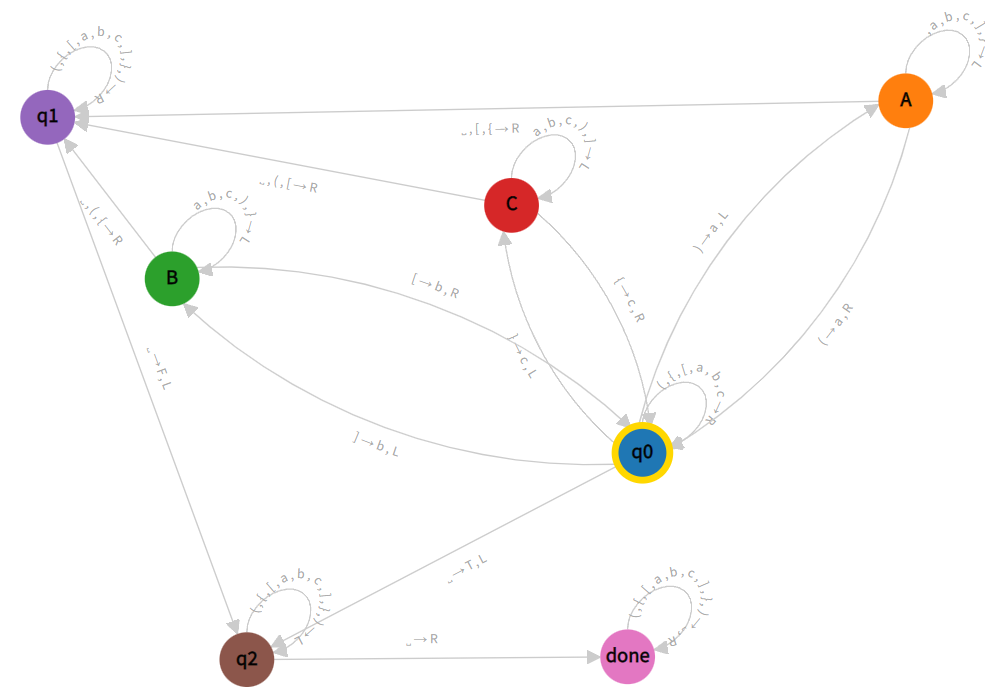
\includegraphics[width=17cm]{pictures/2.2.png}
\end{figure}\\ 
\ Примеры:\\
\ '$($ $[$ $($ $[$ $]$ $)$ $]$ $)$' -> T \\
\ '$($ $)$ $[$ $]$ \{ \}' -> T \\
\ '$($ $($ )$ $[$ $]$ \{\}$)' -> T \\
\ '$($ $[$ $($ $]$ $)$' -> F \\
\ '$($ $($ \{ $[$ $]$ \} $($ $[$ $]$ $)$' -> F \\
\ '$($ $($ $($ $)$ $)$' -> F\\
\\ \\
Алгоритм: \\
С самого начала мы пропускаем все открывающие скобки. Дойдя до первой закрывающей, мы заменяем ее на соответствующую букву. Затем сдвигаемся влево до тех пор, пока не найдется такая же открывающая скобка. Заменяем ее на ту же букву. Так происходит со всеми скобками. Если мы дошли до начала слова, не найдя открывающей скобки, переходим в терминальное состояние, записав F. Если все хорошо, то доходим до начала слова и начинаем идти вправо, пропуская буквы. Если попадается незатронутая скобка, значит, у нее нет закрывающей пары. Тогда переходим в терминальное состояние, записав F. Если попадаются только буквы, то переходим в терминальное состояние, записав T. В терминальном состоянии мы очищаем с ленты все, что идет левее буквы F или T.

\newpage
    \item Поиск минимального по длине слова в строке (слова состоят из символов 1 и 0 и разделены пробелом)
   \begin{figure}[h]
        \centering
        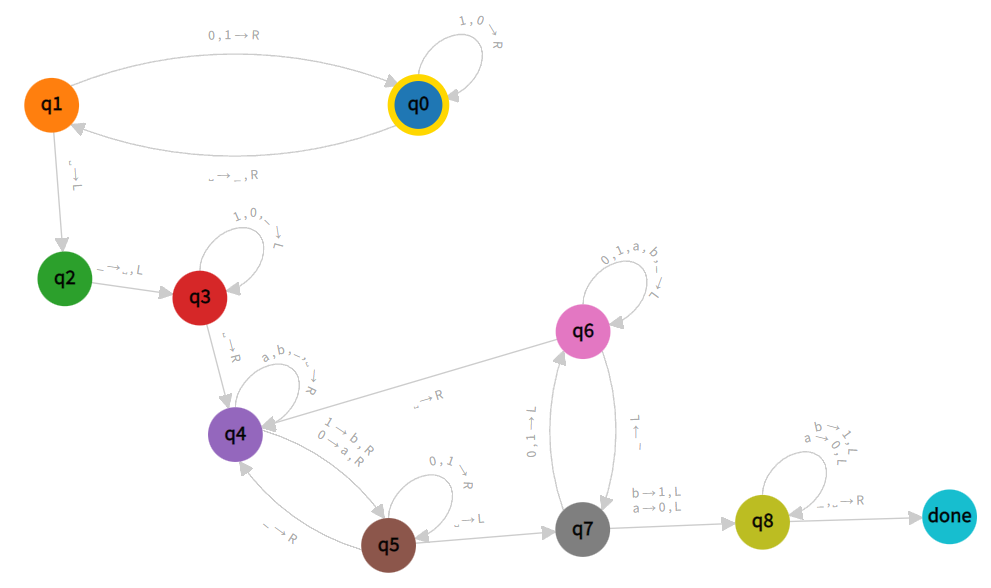
\includegraphics[width=15cm]{pictures/2.3.png}
   \end{figure}\\ \\
   
Алгоритм:\\
Мы заменяем по одной цифре из каждого слова на буквы. Так мы делаем до тех пор, пока одно из слов не будет состоять только из букв. Если мы остановим замены в этот момент, то это слово и будет самым коротким. Тогда мы проходим по нему, заменив буквы обратно на цифры. Затем мы останавливаем курсор МТ в начале этого слова.
\\ 
\ Алгоритм останавливает выполнение в начала искомого слова, т.е. он не выделяет это слово, удалив остальные.
\\ \\
\end{enumerate}\\
% КОНЕЦ ЗАДАНИЯ 2


% НАЧАЛО ЗАДАНИЯ 3
\section{Квантовые вычисления}

\subsection{Генерация суперпозиций 1}

Дано $N$ кубитов ($1 \le N \le 8$) в нулевом состоянии $\Ket{0\dots0}$. Также дана некоторая последовательность битов, которое задаёт ненулевое базисное состояние размера $N$. Задача получить суперпозицию нулевого состояния и заданного.

$$\Ket{S} = \frac{1}{\sqrt2}(\Ket{0\dots0} +\Ket{\psi})$$

То есть требуется реализовать операцию, которая принимает на вход:

\begin{enumerate}
    \item Массив кубитов $q_s$
    \item Массив битов $bits$ описывающих некоторое состояние $\Ket{\psi}$. Это массив имеет тот же самый размер, что и $qs$. Первый элемент этого массива равен $1$.
\end{enumerate}\\
Решение:\\
Будем испольщовать пакет qiskit для Python.\\
Функции, необходимые для решения задачи:
Для первого кубита всегда применяем оператор Адамара. Затем смотрим на вектор bits, если кубит равен 1, то мы спутываем его с первым кубитом.
\begin{figure}[h]
        \centering
        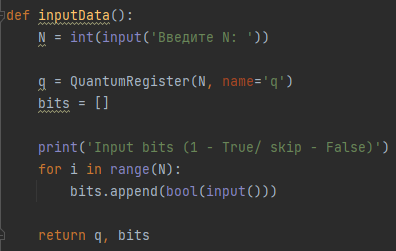
\includegraphics{pictures/Code3.1.png}
   \end{figure} \\ \\ \\ \\ \\ \\ \\ 

Основной код программы:
\begin{figure}[h]
        \centering
        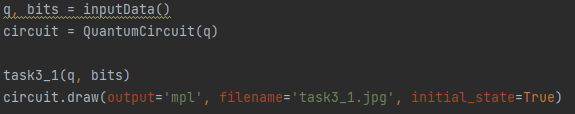
\includegraphics{pictures/main3.1.png}
   \end{figure} \\ 

Тест при N = 4:
\begin{figure}[h]
        \centering
        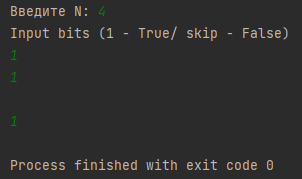
\includegraphics{pictures/test3.1.png}
   \end{figure} \\ 
   
Результат:
\begin{figure}[h]
        \centering
        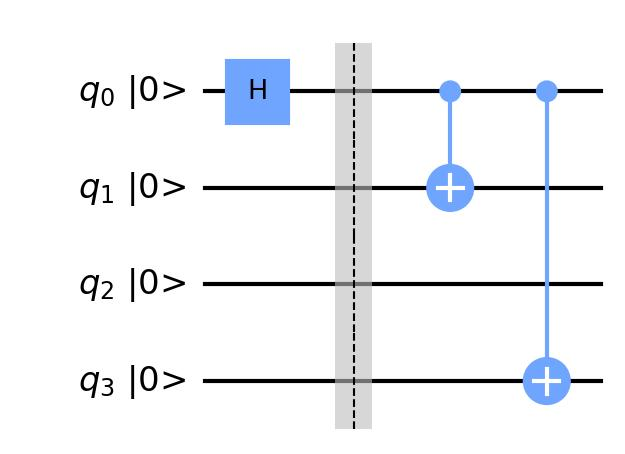
\includegraphics{pictures/task3_1.jpg}
   \end{figure} \\ \\ \\ \\ \\ \\ \\ 

\subsection{Различение состояний 1}

Дано $N$ кубитов ($1 \le N \le 8$), которые могут быть в одном из двух состояний:

$$\Ket{GHZ} = \frac{1}{\sqrt2}(\Ket{0\dots0} +\Ket{1\dots1})$$
$$\Ket{W} = \frac{1}{\sqrt N}(\Ket{10\dots00}+\Ket{01\dots00} + \dots +\Ket{00\dots01})$$

Требуется выполнить необходимые преобразования, чтобы точно различить эти два состояния. Возвращать $0$, если первое состояние и 1, если второе. 
\\\\
На вход процедура получает  кубитов. Для различения состояний пользуемся следующими соображениями:\\

Первое состояние при измерении дает все кубиты либо 1, либо 0.\\

Второе состояние при измерении дает только один купит 1, остальные 0.\\ \\

Кроме того, нуобходимо учитывать случай N = 1:
$$\Ket{GHZ} = \frac{1}{\sqrt2}(\Ket{0} +\Ket{1})$$
$$\Ket{W} = \Ket{1}$$\\

Тогда мы сначала измеряем кубиты, учитываем N = 1. Если количество кубитов равно единице, и заданное состояние равно $\Ket{1}$, то сразу определяем его как второе состояние, иначе - как первое. Если кол-во кубитов >1, то считаем единичные кубиты, полученные после измерения. Если в результате имеем только один единичный кубит, то определили второе состояние, иначе - первое.\\
Решение:\\
Функция ввода и создания векторов состояний: \\
\begin{figure}[h]
        \centering
        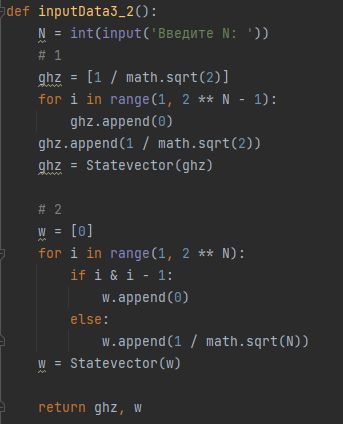
\includegraphics{pictures/input3.2.png}
   \end{figure}\\
Функция, реализующая алгоритм: \\
\begin{figure}[h]
        \centering
        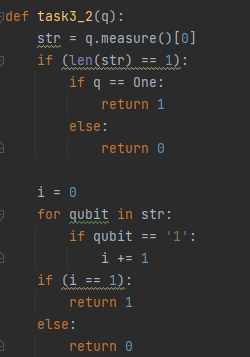
\includegraphics{pictures/task3.2.png}
   \end{figure}\\ \\ \\ \\ 
Основной код: \\
\begin{figure}[h]
        \centering
        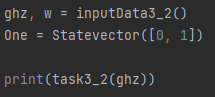
\includegraphics{pictures/main3.2.png}
   \end{figure}\\
Тест: \\
\begin{figure}[h]
        \centering
        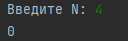
\includegraphics{pictures/test3.2.png}
   \end{figure}\\

\subsection{Различение состояний 2}

Дано $2$ кубита, которые могут быть в одном из двух состояний:

$$\Ket{S_0} = \frac{1}{2}(\Ket{00} + \Ket{01} + \Ket{10} + \Ket{11})$$
$$\Ket{S_1} = \frac{1}{2}(\Ket{00} - \Ket{01} + \Ket{10} - \Ket{11})$$
$$\Ket{S_2} = \frac{1}{2}(\Ket{00} + \Ket{01} - \Ket{10} - \Ket{11})$$
$$\Ket{S_3} = \frac{1}{2}(\Ket{00} - \Ket{01} - \Ket{10} + \Ket{11})$$


Требуется выполнить необходимые преобразования, чтобы точно различить эти четыре состояния. Возвращать требуется индекс состояния (от $0$ до $3$). 
\\\\
Решение:\\
Сначала создаем состояния:\\
\begin{figure}[h]
        \centering
        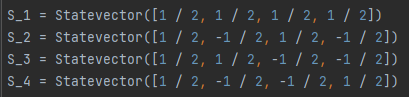
\includegraphics{pictures/states3.3.png}
   \end{figure}\\
Алгоритм будет основываться на том, чтобы применить оператор Адамара для каждого из 2-х кубитов. У нас получиться 4 различных состояния, которые мы впоследствии измерим.\\
Матрица оператора Адамара для 2-х кубитов:\\
\begin{equation*}
H^2 = \frac{1}{2}\left(
\begin{array}{cccc}
1 & 1 & 1 & 1\\
1 & -1 & 1 & -1\\
1 & 1 & -1 & -1\\
1 & -1 & -1 & 1
\end{array}
\right)
\end{equation*} \\

Переведем операторы состояния в векторный вид и применим оператор Адамара:\\
\begin{equation*}
H^2\Ket{S_1} = \frac{1}{2}\left(
\begin{array}{cccc}
1 & 1 & 1 & 1\\
1 & -1 & 1 & -1\\
1 & 1 & -1 & -1\\
1 & -1 & -1 & 1
\end{array}
\right) \frac{1}{2}\left( \begin{array} {c}
1 & 1 & 1 & 1
\end{array}
\right) = \frac{1}{4}\left(
\begin{array}{cccc}
1 + 1 + 1 + 1\\
1 - 1 + 1 - 1\\
1 + 1 - 1 - 1\\
1 - 1  -1 + 1
\end{array}
\right) = \frac{1}{4}\left( \begin{array} {c}
4 & 0 & 0 & 0
\end{array}
\right) = \left( \begin{array} {c}
1 & 0 & 0 & 0
\end{array}
\right)
\end{equation*} \\

Аналогично для других состояний:\\
\begin{equation*}
\Ket{S_1} = \left( \begin{array} {c}
1 & 0 & 0 & 0
\end{array}
\right);
\Ket{S_2} = \left( \begin{array} {c}
0 & 1 & 0 & 0
\end{array}
\right);
\Ket{S_3} = \left( \begin{array} {c}
0 & 0 & 1 & 0
\end{array}
\right);
\Ket{S_4} = \left( \begin{array} {c}
0 & 0 & 0 & 1
\end{array}
\right)
\end{equation*} \\

Переведем состояния обратно. Получим:\\
\begin{equation*}
\Ket{S_1} = \Ket{00};
\Ket{S_2} = \Ket{01};
\Ket{S_3} = \Ket{10};
\Ket{S_4} = \Ket{11}
\end{equation*} \\

\newpage
Напишем функцию для определения состояния:\\
\begin{figure}[h]
        \centering
        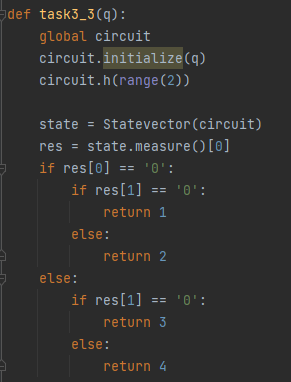
\includegraphics{pictures/task3.3.png}
   \end{figure}\\ \\ \\
   
Основной код программы:\\
\begin{figure}[h]
        \centering
        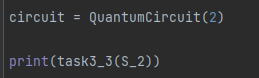
\includegraphics{pictures/main3.3.png}
   \end{figure}\\
   
Результат теста:\\
\begin{figure}[h]
        \centering
        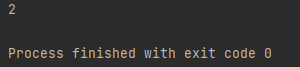
\includegraphics{pictures/test3.3.png}
   \end{figure}\\

\end{document}

